\documentclass[12pt]{article}

\usepackage{tikz}
\usetikzlibrary{plotmarks}
\begin{document}

% PGF/TikZ picture from SSJ: Piecewise linearization
% XScale = 100.0,  YScale = 100.0,  XShift = -2.2,  YShift = -1.1
% Therefore, thisFileXValue = (originalSeriesXValue+XShift)*XScale
%        and thisFileYValue = (originalSeriesYValue+YShift)*YScale

\begin{figure}
\begin{center}
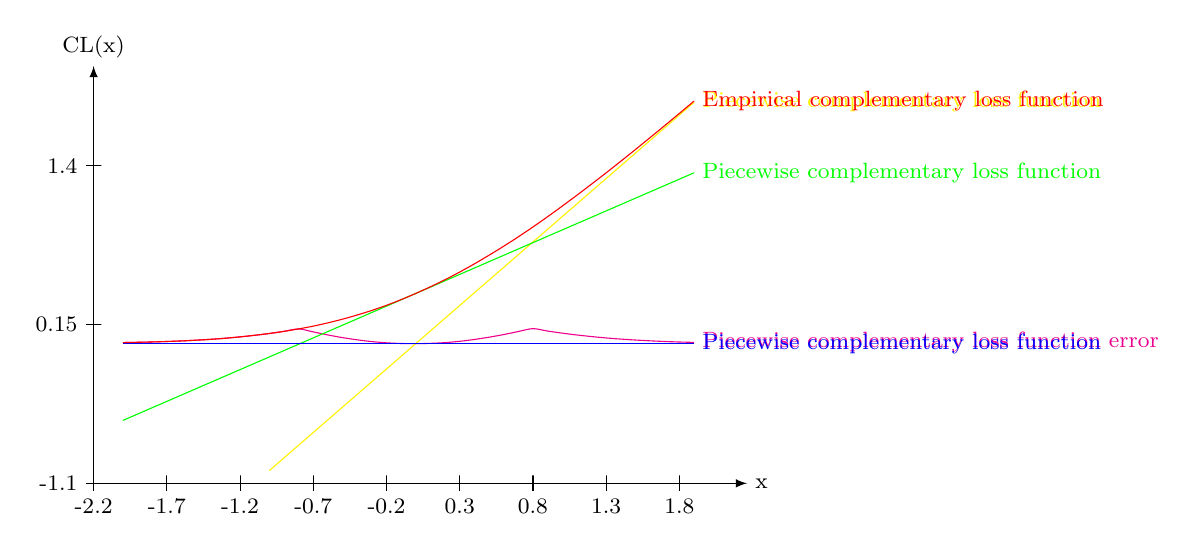
\begin{tikzpicture}[x=0.018604651162790697cm, y=0.016129032258064516cm]
\footnotesize
\draw [-latex] ([xshift=-0mm] 0.0,0) -- ([xshift=3mm] 430.00000000000006,0) node[right] {x};
\draw (0.0,0) -- +(0mm,1mm) -- +(0mm,-1mm) node[below] {-2.2};
\draw (50.0,0) -- +(0mm,1mm) -- +(0mm,-1mm) node[below] {-1.7};
\draw (100.0,0) -- +(0mm,1mm) -- +(0mm,-1mm) node[below] {-1.2};
\draw (150.0,0) -- +(0mm,1mm) -- +(0mm,-1mm) node[below] {-0.7};
\draw (200.0,0) -- +(0mm,1mm) -- +(0mm,-1mm) node[below] {-0.2};
\draw (250.0,0) -- +(0mm,1mm) -- +(0mm,-1mm) node[below] {0.3};
\draw (300.0,0) -- +(0mm,1mm) -- +(0mm,-1mm) node[below] {0.8};
\draw (350.0,0) -- +(0mm,1mm) -- +(0mm,-1mm) node[below] {1.3};
\draw (400.0,0) -- +(0mm,1mm) -- +(0mm,-1mm) node[below] {1.8};
\draw [-latex] ([yshift=-0mm] 0,0.0) -- ([yshift=3mm] 0, 310.0) node[above] {CL(x)};
\draw (0,0.0) -- +(1mm,0mm) -- +(-1mm,0mm) node[left] {-1.1};
\draw (0,125.0) -- +(1mm,0mm) -- +(-1mm,0mm) node[left] {0.15};
\draw (0,250.0) -- +(1mm,0mm) -- +(-1mm,0mm) node[left] {1.4};
\draw [smooth, color=magenta, mark= , style=solid] plot coordinates {%
(20.00,110.8354) %   (-2.000000,  0.008354)
(30.00,111.0732) %   (-1.900000,  0.010732)
(40.00,111.3426) %   (-1.800000,  0.013426)
(50.00,111.6992) %   (-1.700000,  0.016992)
(60.00,112.1500) %   (-1.600000,  0.021500)
(70.00,112.7191) %   (-1.500000,  0.027191)
(80.00,113.4170) %   (-1.400000,  0.034170)
(90.00,114.2698) %   (-1.300000,  0.042698)
(100.00,115.3424) %   (-1.200000,  0.053424)
(110.00,116.5795) %   (-1.100000,  0.065795)
(120.00,118.0093) %   (-1.000000,  0.080093)
(130.00,119.6816) %   (-0.900000,  0.096816)
(140.00,121.6023) %   (-0.800000,  0.116023)
(150.00,119.2502) %   (-0.700000,  0.092502)
(160.00,116.8354) %   (-0.600000,  0.068354)
(170.00,114.7408) %   (-0.500000,  0.047408)
(180.00,113.0227) %   (-0.400000,  0.030227)
(190.00,111.6180) %   (-0.300000,  0.016180)
(200.00,110.6540) %   (-0.200000,  0.006540)
(210.00,110.1311) %   (-0.100000,  0.001311)
(220.00,110.0089) %   (0.000000,  0.000089)
(230.00,110.2386) %   (0.100000,  0.002386)
(240.00,110.8198) %   (0.200000,  0.008198)
(250.00,111.8541) %   (0.300000,  0.018541)
(260.00,113.3002) %   (0.400000,  0.033002)
(270.00,115.0760) %   (0.500000,  0.050760)
(280.00,117.1616) %   (0.600000,  0.071616)
(290.00,119.5548) %   (0.700000,  0.095548)
(300.00,121.8200) %   (0.800000,  0.118200)
(310.00,119.9118) %   (0.900000,  0.099118)
(320.00,118.2659) %   (1.000000,  0.082659)
(330.00,116.8297) %   (1.100000,  0.068297)
(340.00,115.5753) %   (1.200000,  0.055753)
(350.00,114.4918) %   (1.300000,  0.044918)
(360.00,113.5919) %   (1.400000,  0.035919)
(370.00,112.8519) %   (1.500000,  0.028519)
(380.00,112.2277) %   (1.600000,  0.022277)
(390.00,111.6971) %   (1.700000,  0.016971)
(400.00,111.2912) %   (1.800000,  0.012912)
(410.00,110.9874)} %   (1.900000,  0.009874)
 node[right] {Piecewise complementary loss function error};
\draw [smooth, color=yellow, mark= , style=solid] plot coordinates {%
(120.00,10.0628) %   (-1.000000,  -0.999372)
(130.00,20.0628) %   (-0.900000,  -0.899372)
(140.00,30.0628) %   (-0.800000,  -0.799372)
(150.00,40.0628) %   (-0.700000,  -0.699372)
(160.00,50.0628) %   (-0.600000,  -0.599372)
(170.00,60.0628) %   (-0.500000,  -0.499372)
(180.00,70.0628) %   (-0.400000,  -0.399372)
(190.00,80.0628) %   (-0.300000,  -0.299372)
(200.00,90.0628) %   (-0.200000,  -0.199372)
(210.00,100.0628) %   (-0.100000,  -0.099372)
(220.00,110.0628) %   (0.000000,  0.000628)
(230.00,120.0628) %   (0.100000,  0.100628)
(240.00,130.0628) %   (0.200000,  0.200628)
(250.00,140.0628) %   (0.300000,  0.300628)
(260.00,150.0628) %   (0.400000,  0.400628)
(270.00,160.0628) %   (0.500000,  0.500628)
(280.00,170.0628) %   (0.600000,  0.600628)
(290.00,180.0628) %   (0.700000,  0.700628)
(300.00,190.0628) %   (0.800000,  0.800628)
(310.00,200.0628) %   (0.900000,  0.900628)
(320.00,210.0628) %   (1.000000,  1.000628)
(330.00,220.0628) %   (1.100000,  1.100628)
(340.00,230.0628) %   (1.200000,  1.200628)
(350.00,240.0628) %   (1.300000,  1.300628)
(360.00,250.0628) %   (1.400000,  1.400628)
(370.00,260.0628) %   (1.500000,  1.500628)
(380.00,270.0628) %   (1.600000,  1.600628)
(390.00,280.0628) %   (1.700000,  1.700628)
(400.00,290.0628) %   (1.800000,  1.800628)
(410.00,300.0628)} %   (1.900000,  1.900628)
 node[right] {Piecewise complementary loss function};
\draw [smooth, color=green, mark= , style=solid] plot coordinates {%
(20.00,49.5519) %   (-2.000000,  -0.604481)
(30.00,54.5519) %   (-1.900000,  -0.554481)
(40.00,59.5519) %   (-1.800000,  -0.504481)
(50.00,64.5519) %   (-1.700000,  -0.454481)
(60.00,69.5519) %   (-1.600000,  -0.404481)
(70.00,74.5519) %   (-1.500000,  -0.354481)
(80.00,79.5519) %   (-1.400000,  -0.304481)
(90.00,84.5519) %   (-1.300000,  -0.254481)
(100.00,89.5519) %   (-1.200000,  -0.204481)
(110.00,94.5519) %   (-1.100000,  -0.154481)
(120.00,99.5519) %   (-1.000000,  -0.104481)
(130.00,104.5519) %   (-0.900000,  -0.054481)
(140.00,109.5519) %   (-0.800000,  -0.004481)
(150.00,114.5519) %   (-0.700000,  0.045519)
(160.00,119.5519) %   (-0.600000,  0.095519)
(170.00,124.5519) %   (-0.500000,  0.145519)
(180.00,129.5519) %   (-0.400000,  0.195519)
(190.00,134.5519) %   (-0.300000,  0.245519)
(200.00,139.5519) %   (-0.200000,  0.295519)
(210.00,144.5519) %   (-0.100000,  0.345519)
(220.00,149.5519) %   (0.000000,  0.395519)
(230.00,154.5519) %   (0.100000,  0.445519)
(240.00,159.5519) %   (0.200000,  0.495519)
(250.00,164.5519) %   (0.300000,  0.545519)
(260.00,169.5519) %   (0.400000,  0.595519)
(270.00,174.5519) %   (0.500000,  0.645519)
(280.00,179.5519) %   (0.600000,  0.695519)
(290.00,184.5519) %   (0.700000,  0.745519)
(300.00,189.5519) %   (0.800000,  0.795519)
(310.00,194.5519) %   (0.900000,  0.845519)
(320.00,199.5519) %   (1.000000,  0.895519)
(330.00,204.5519) %   (1.100000,  0.945519)
(340.00,209.5519) %   (1.200000,  0.995519)
(350.00,214.5519) %   (1.300000,  1.045519)
(360.00,219.5519) %   (1.400000,  1.095519)
(370.00,224.5519) %   (1.500000,  1.145519)
(380.00,229.5519) %   (1.600000,  1.195519)
(390.00,234.5519) %   (1.700000,  1.245519)
(400.00,239.5519) %   (1.800000,  1.295519)
(410.00,244.5519)} %   (1.900000,  1.345519)
 node[right] {Piecewise complementary loss function};
\draw [smooth, color=blue, mark= , style=solid] plot coordinates {%
(20.00,110.0000) %   (-2.000000,  0.000000)
(30.00,110.0000) %   (-1.900000,  0.000000)
(40.00,110.0000) %   (-1.800000,  0.000000)
(50.00,110.0000) %   (-1.700000,  0.000000)
(60.00,110.0000) %   (-1.600000,  0.000000)
(70.00,110.0000) %   (-1.500000,  0.000000)
(80.00,110.0000) %   (-1.400000,  0.000000)
(90.00,110.0000) %   (-1.300000,  0.000000)
(100.00,110.0000) %   (-1.200000,  0.000000)
(110.00,110.0000) %   (-1.100000,  0.000000)
(120.00,110.0000) %   (-1.000000,  0.000000)
(130.00,110.0000) %   (-0.900000,  0.000000)
(140.00,110.0000) %   (-0.800000,  0.000000)
(150.00,110.0000) %   (-0.700000,  0.000000)
(160.00,110.0000) %   (-0.600000,  0.000000)
(170.00,110.0000) %   (-0.500000,  0.000000)
(180.00,110.0000) %   (-0.400000,  0.000000)
(190.00,110.0000) %   (-0.300000,  0.000000)
(200.00,110.0000) %   (-0.200000,  0.000000)
(210.00,110.0000) %   (-0.100000,  0.000000)
(220.00,110.0000) %   (0.000000,  0.000000)
(230.00,110.0000) %   (0.100000,  0.000000)
(240.00,110.0000) %   (0.200000,  0.000000)
(250.00,110.0000) %   (0.300000,  0.000000)
(260.00,110.0000) %   (0.400000,  0.000000)
(270.00,110.0000) %   (0.500000,  0.000000)
(280.00,110.0000) %   (0.600000,  0.000000)
(290.00,110.0000) %   (0.700000,  0.000000)
(300.00,110.0000) %   (0.800000,  0.000000)
(310.00,110.0000) %   (0.900000,  0.000000)
(320.00,110.0000) %   (1.000000,  0.000000)
(330.00,110.0000) %   (1.100000,  0.000000)
(340.00,110.0000) %   (1.200000,  0.000000)
(350.00,110.0000) %   (1.300000,  0.000000)
(360.00,110.0000) %   (1.400000,  0.000000)
(370.00,110.0000) %   (1.500000,  0.000000)
(380.00,110.0000) %   (1.600000,  0.000000)
(390.00,110.0000) %   (1.700000,  0.000000)
(400.00,110.0000) %   (1.800000,  0.000000)
(410.00,110.0000)} %   (1.900000,  0.000000)
 node[right] {Piecewise complementary loss function};
\draw [smooth, color=red, mark= , style=solid] plot coordinates {%
(20.00,110.8354) %   (-2.000000,  0.008354)
(30.00,111.0732) %   (-1.900000,  0.010732)
(40.00,111.3426) %   (-1.800000,  0.013426)
(50.00,111.6992) %   (-1.700000,  0.016992)
(60.00,112.1500) %   (-1.600000,  0.021500)
(70.00,112.7191) %   (-1.500000,  0.027191)
(80.00,113.4170) %   (-1.400000,  0.034170)
(90.00,114.2698) %   (-1.300000,  0.042698)
(100.00,115.3424) %   (-1.200000,  0.053424)
(110.00,116.5795) %   (-1.100000,  0.065795)
(120.00,118.0093) %   (-1.000000,  0.080093)
(130.00,119.6816) %   (-0.900000,  0.096816)
(140.00,121.6023) %   (-0.800000,  0.116023)
(150.00,123.8021) %   (-0.700000,  0.138021)
(160.00,126.3872) %   (-0.600000,  0.163872)
(170.00,129.2926) %   (-0.500000,  0.192926)
(180.00,132.5745) %   (-0.400000,  0.225745)
(190.00,136.1699) %   (-0.300000,  0.261699)
(200.00,140.2059) %   (-0.200000,  0.302059)
(210.00,144.6829) %   (-0.100000,  0.346829)
(220.00,149.5608) %   (0.000000,  0.395608)
(230.00,154.7904) %   (0.100000,  0.447904)
(240.00,160.3717) %   (0.200000,  0.503717)
(250.00,166.4059) %   (0.300000,  0.564059)
(260.00,172.8521) %   (0.400000,  0.628521)
(270.00,179.6278) %   (0.500000,  0.696278)
(280.00,186.7135) %   (0.600000,  0.767135)
(290.00,194.1067) %   (0.700000,  0.841067)
(300.00,201.8828) %   (0.800000,  0.918828)
(310.00,209.9746) %   (0.900000,  0.999746)
(320.00,218.3287) %   (1.000000,  1.083287)
(330.00,226.8925) %   (1.100000,  1.168925)
(340.00,235.6381) %   (1.200000,  1.256381)
(350.00,244.5546) %   (1.300000,  1.345546)
(360.00,253.6547) %   (1.400000,  1.436547)
(370.00,262.9147) %   (1.500000,  1.529147)
(380.00,272.2905) %   (1.600000,  1.622905)
(390.00,281.7599) %   (1.700000,  1.717599)
(400.00,291.3540) %   (1.800000,  1.813540)
(410.00,301.0502)} %   (1.900000,  1.910502)
 node[right] {Empirical complementary loss function};
\end{tikzpicture}
\end{center}
\caption{Piecewise linearization}
\end{figure}
\end{document}
